\section{실패 사례 분석}

\begin{figure*}[!t]
\centering
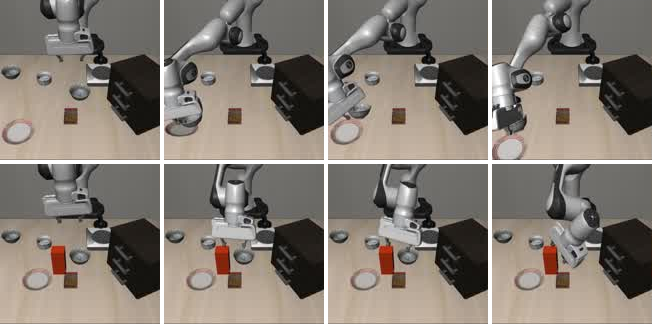
\includegraphics[width=0.72\textwidth]{figures/arm_failure_frames.png}
\caption{로봇팔 실패 사례(0, 2, 4, 7초). (위) 접시를 멀리 둔 장면: 그릇을 들어 운반하지만 접시 위에 놓지 못함.
(아래) 높이 15\,cm 장애물 장면: 그리퍼가 장애물에 걸려 그릇에 접근하지 못함.}\label{fig:arm}
\end{figure*}

\subsection*{로봇팔: 접근 차단 충돌과 PASS/FAIL 경계}
그림~\ref{fig:arm}은 대표 실패 장면이다. 실험 1의 FAIL 7건은 모두 제한 시간(약 15초) 안에 성공하지 못했고, 그릇은 전혀 들리지 않았으며
로봇과 장애물의 접촉이 10--14초 지속되었다. 반면 PASS는 약 5초 만에 끝나며 그릇이 15--17\,cm
들렸다가 접시 중심 2\,cm 이내에 놓였다. 즉 실패는 운반 중 충돌이 아니라 \textbf{잡기 전 접근 단계의
충돌}이다. AFS는 첫 실패의 접촉 기록을 읽고 장애물을 이송 경로 중앙에 크게 배치하는 방향으로
수렴하였다.

같은 정책으로 장애물 높이와 목표 거리를 단계적으로 바꾼 통제 실험(11개 장면)에서 명확한
경계가 확인되었다. 장애물 높이 10·12\,cm에서는 PASS, 14·15·17\,cm에서는 모두 FAIL이었고
최대 접촉력은 198--279\,N이었다. 접시를 기존 위치에서 이동 경로의 37.5\%까지 옮기면 PASS,
50\%에서는 그릇을 들고 운반했지만 접시 8.7\,cm 앞에서 놓지 못해 FAIL이었다.
따라서 이 정책의 안전 운용 경계는 \textbf{장애물 높이 12--14\,cm}, \textbf{목표 이동 37.5--50\%} 구간에 있다.

\subsection*{휴머노이드: 목표 위치 점유}
기준 장면 PASS(최종 목표 거리 0.116\,m) 뒤, AFS는 상자의 횡방향 위치만 1.0에서 0.0으로 바꿨다.
상자가 목표 영역을 점유하자 경로 계획기는 목표점이 막혀 있다며 목표 접근 요청을 거절했고,
상자 밀기 요청은 로봇이 상자 면과 약 90도 어긋난 방향에 있어 실행 전에 거절되었다.
로봇은 목표 0.86\,m 앞에서 허용된 행동 결정 10회를 모두 소진하였다. 두 축(상자 횡·종방향)을 바꾼
다른 FAIL에서도 목표점 거절과 우회 경로 차단이 반복되어 목표 0.43\,m 앞에서 종료되었다.
두 사례 모두 단순한 환경 변화가 경로 계획과 물체 밀기 기능의 한계를 드러낸 경우다.
